\documentclass[a4paper, 12pt, fleqn]{article}
\usepackage[czech]{babel}
\usepackage[utf8x]{inputenc}
\usepackage[T1]{fontenc}
%\usepackage[latin2]{inputenc} % pro iso8859-2
%\usepackage[IL2]{fontenc}     % fonty vygenerované pro iso8859-2

%%%%%%%%%%%%%%%%%%%%%%%%%%%%%%%%%%%%%%%%%%%%%%%%%%%%%%%%%%%%%%%%%%%%%%%%%
%% Hlavička ZDE VYPLNIT 
\newcommand{\autor}{Daniel KARLÍK, Michaela MAŠKOVÁ}
\newcommand{\cislomp}{1} % 1,2,3
\newcommand{\zadani}{OVM model}
\newcommand{\rocnik}{2020/2021}
%% Konec hlavičky
%%%%%%%%%%%%%%%%%%%%%%%%%%%%%%%%%%%%%%%%%%%%%%%%%%%%%%%%%%%%%%%%%%%%%%%%%


%\usepackage{enumitem} 
%\setlist{noitemsep, nolistsep}

\usepackage{calc}
\setlength{\textheight}{10in}
\setlength{\textwidth}{6.5in}
\setlength\oddsidemargin{0cm}
\setlength\evensidemargin{(0cm}
\setlength\topmargin{(\paperheight-\textheight-\headheight-\headsep-\footskip)/2 - 1in}

%% matematika
\usepackage{amssymb}
\usepackage{amsmath}

%% grafika
\usepackage{color}
\usepackage{tikz}
\usetikzlibrary{decorations.pathreplacing, patterns}
\usetikzlibrary{arrows.meta,positioning, datavisualization}
\usepackage{graphicx}
%\usepackage{animate}
\usepackage{booktabs}

%% plots
\usepackage{pgfplots}
\pgfplotsset{compat=1.16}
\usepackage{caption}
\usepackage{subcaption}

%% Nastavení grafiky matlabovských kódů ------------------------------------------------
\usepackage{verbatim}
\usepackage{listings} % balíček pro blok kódu
\usepackage{matlab-prettifier} % matlabovské barvičky atd.
\renewcommand{\lstlistingname}{Kód} % úprava caption
% nějaké další drobnosti
\lstset{basicstyle=\mlttfamily}
\lstset{frame=single}
\lstset{numbers=left}

% pro případ použití speciálních českých znaků v kódu (např. v komentáři)
\lstset{literate=
	{í}{{\'i}}1
	{á}{{\'a}}1
	{ý}{{\'y}}1
	{é}{{\'e}}1
	{ř}{{\v{r}}}1
	{ó}{{\'o}}1
	{ů}{{\r{u}}}1
	{č}{{\v{c}}}1
	{ě}{{\v{e}}}1
	{ž}{{\v{z}}}1
}

% ---------------------------------------------------------------------------------------
\begin{document}
%%%%%%%%%%%%%%%%%%%%%%%%%%%%%%%%%%%%%%%%%%%%%%%%%%%%%%%%%%%%%%%%%%%%%%%%%%%%%%%%
%% Vysázení hlavičky - NEMĚNIT
\hrule
\medskip
\noindent{\Large \textbf{01SSI} -- Miniprojekt číslo \cislomp\hfill\rocnik}
\hrule
\medskip
{\large
\noindent
\begin{tabular}{lp{12cm}}
Posluchači:& \textbf{\autor}\\
Zadání:& \textbf{\zadani} \\
\end{tabular}

\medskip
\noindent
 \hspace{2mm}Odevzdáno: \hfill Získané body: \hfill Finální: ANO/NE
}
\medskip
\hrule
%% Konec vysázení hlavičky
%%%%%%%%%%%%%%%%%%%%%%%%%%%%%%%%%%%%%%%%%%%%%%%%%%%%%%%%%%%%%%%%%%%%%%%%%%%%%%%%%%%%

%% Vlastní popis

\section{Teoretický úvod}

\subsection{Optimal Velocity Model}
% new commands
\newcommand{\vopt}{v_{opt}}
\newcommand{\va}{v_{\alpha}}
\newcommand{\dva}{\dot{v}_{\alpha}}
\newcommand{\Sa}{S_{\alpha}}
\newcommand{\X}{\mathbb{X}}
\newcommand{\V}{\mathbb{V}}
\newcommand{\da}{d_{\alpha}}
\newcommand{\vmax}{v_{max}}
\newcommand{\dsafe}{d_{safe}}
\newcommand{\der}{\mathrm{d}}
%\newcommand[1]{\hev}{\Theta (#1)}

Optimal Velocity model je zobecněním car-following modelu FLM -- \textit{Follow the Leader Model}. Cílem každého vozidla je dosáhnout a udržovat si svoji optimální rychlost $\vopt$. Optimální rychlost se bude měnit tak, že pokud
\begin{itemize}
	\item $\va > \vopt \implies $ vozidlo zpomalí, tedy $ \dva < 0$
	\item $\va < \vopt \implies $ vozidlo zrychlí, tedy $ \dva > 0$.
\end{itemize}
Zrychlení definujeme jako
\begin{equation}
	\dva = \Sa(\vopt(\X, \V) - \va),
	\label{Eq: Zrychlení}
\end{equation}
kde parametr $\Sa$ je konstanta, která kontroluje rychlost reakce (změny rychlosti). Samotná optimální rychlost pak bude funkcí vzdálenosti $\da$ (vzdálenost od předchozího vozidla), tedy $\vopt(\X, \V) = \vopt(\da)$, a bude splňovat následující podmínky:
\begin{itemize}
	\item $\vopt(d) \xrightarrow{d \rightarrow 0^{+}} 0$
	\item $\vopt(d) \xrightarrow{d \rightarrow +\infty} \vmax$
	\item $\vopt(d)$ je neklesající (resp. rostoucí) funkcí.
\end{itemize}

Z výše uvedeného je tak jasné, že kvalita a vlastnosti modelu budou záviset na volbě funkce $\vopt(d)$. Pro ilustraci těchto vlastností tak byly zvoleny různé funkce.

\subsection{Vybrané funkce $\vopt$}
Už jsme naznačili, jaký má být trend funkce $\vopt$. Musí se jednat o funkci rostoucí (neklesající), která je omezená zdola 0 a shora maximální možnou rychlostí.

Nejjednoduší volbou je funkce
\begin{equation}
	\vopt^1(x) = \vmax \Theta (\Delta x - \dsafe),
	\label{Eq: v1}
\end{equation}
kde $\Delta x = x_{\alpha} - x_{\alpha - 1}$. Její graf je na Obr. \ref{Obr: v1}.

\begin{figure}
	\centering
	\begin{tikzpicture}
		\draw[-latex] (0,0) -- (0,5);
		\draw[-latex] (0,0) -- (10,0);
		\draw[-, color=blue, line width=0.5mm] (0,0.03) -- (3,0.03);
		\draw[-, color=blue, line width=0.5mm] (3,4) -- (9,4);
		\node[] at (-0.3,-.3) (zero) {0};
		\node[] at (0,5.3) (v) {$\vopt$};
		\node[] at (10.3,0) (x) {$\Delta x$};
		\draw[-] (-0.1,4) -- (0.1,4);
		\node[] at (-0.6,4) (vmax) {$\vmax$};
		\draw[-] (3,-0.1) -- (3,0.1);
		\node[] at (3,-0.5) (dsafe) {$\dsafe$};
		\draw[dashed] (0,4) -- (3,4);
		\draw[dashed] (3,0) -- (3,4);
	\end{tikzpicture}
	\caption{Vizualizace funkce \eqref{Eq: v1}.}
	\label{Obr: v1}
\end{figure}

Další možností je funkce tvaru
\begin{equation}
	\vopt^2(x)=\begin{cases}
	0 & \Delta x < d_A \\
	g(x) & d_A \leq \Delta x \leq d_B \\
	\vmax & d_B < \Delta x,
	\end{cases}
	\label{Eq: v2}
\end{equation}
kde volba funkce $g(x)$ může být například lineární, tedy $g(x) = x$ nebo jiná. Její graf je vidět na Obr. \ref{Obr: v2}. V našem případě použijeme funkce
\begin{align*}
	\vopt^{(2)} & \rightarrow g^{(2)}(x) = ax + b \\
	\vopt^{(3)} & \rightarrow g^{(3)}(x) = a(x+b)^4 + c,
\end{align*}
kde jednotlivé konstanty jsou dopočítány podle zvolených hodnot $\vmax, d_A$ a $d_B$.


\begin{figure}
	\centering
	\begin{tikzpicture}
	\draw[-latex] (0,0) -- (0,5);
	\draw[-latex] (0,0) -- (10,0);
	\draw[-, color=blue, line width=0.5mm] (0,0.03) -- (2,0.03);
	\draw[-, color=blue, line width=0.5mm] (5,4) -- (9,4);
	\draw[-, color=blue, line width=0.5mm] (2,0.03) -- (5,4);
	
	\node[] at (-0.3,-.3) (zero) {0};
	\node[] at (0,5.3) (v) {$\vopt$};
	\node[] at (10.3,0) (x) {$\Delta x$};
	\draw[-] (-0.1,4) -- (0.1,4);
	\node[] at (-0.6,4) (vmax) {$\vmax$};
	\draw[-] (2,-0.1) -- (2,0.1);
	\node[] at (2,-0.5) (da) {$d_A$};
	\draw[-] (5,-0.1) -- (5,0.1);
	\node[] at (5,-0.5) (db) {$d_B$};
	\draw[dashed] (0,4) -- (5,4);
	\draw[dashed] (5,0) -- (5,4);
	\end{tikzpicture}
	\caption{Vizualizace funkce \eqref{Eq: v2} pro $g(x) = ax + b$.}
	\label{Obr: v2}
\end{figure}

Další možnou funkcí je
\begin{equation}
	\vopt^4(x) = \frac{\vmax}{2} \left[ \tanh(x - \dsafe) + \tanh(\dsafe) \right].
	\label{Eq: v4}
\end{equation}
Její výhodou je, že se jedná o hladkou funkci a tedy lépe odpovídá realitě, kdy vozidlo zrychluje postupně a spojitě. Průběh funkce je vidět na Obr. \ref{Obr: v3}.

\begin{figure}
	\centering
	\pgfplotsset{width=10cm,compat=1.9}
	\begin{tikzpicture}[declare function={vopt3(\x)=25/2*(tanh(\x - 30) + tanh(30));}]
	\begin{axis}%
	[ 
	xmin=20,
	xmax=60,
	axis lines = left,
	ytick={0,5,10,15,20,25,30},
	ymax=35,
	samples=500,
	domain=0:100,
	legend style={at={(0.9,0.2)}},
	xlabel = {$\Delta x \; [m]$},
	ylabel = {$v \; [m/s]$}
	]
	\addplot[blue,mark=none, line width=1]   (x,{vopt3(x)});
	\legend{$v_{opt}^4(x)$}
	\end{axis}
	\end{tikzpicture}
	\caption{Vizualizace funkce \eqref{Eq: v4}.}
	\label{Obr: v3}
\end{figure}

Porovnání všech funkcí si můžeme prohlédnout na Obr. \ref{Obr: Porovnání opt funkcí}.

\begin{figure}
	\centering
	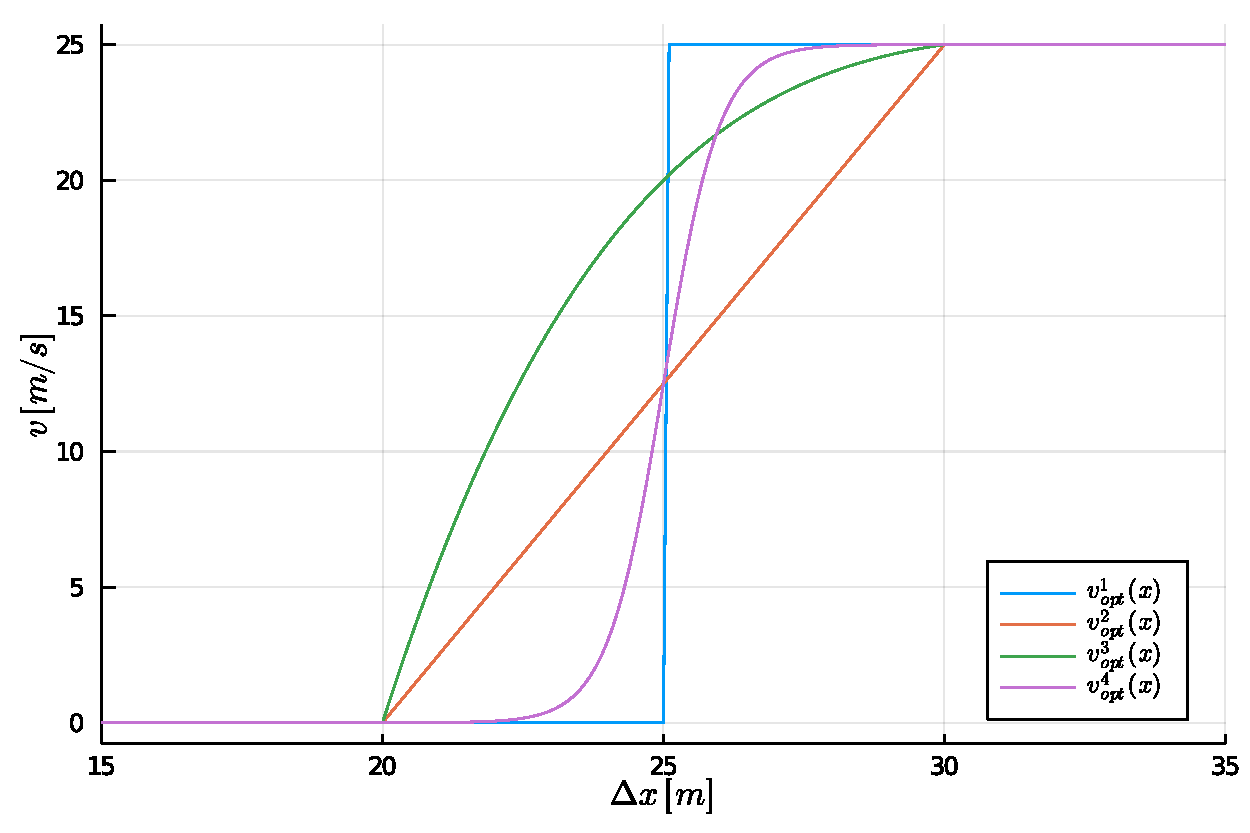
\includegraphics[width=\textwidth]{images/opt_funkce.pdf}
	\caption{Porovnání zvolených funkcí optimální rychlosti.}
	\label{Obr: Porovnání opt funkcí}
\end{figure}

Zároveň si můžeme povšimnout, že chování celého modelu se bude odvíjet i od nastavení jednotlivých konstant. V případě špatně zvolených parametrů se může stát, že simulace nebude funkční.

\subsection{Postup}
Nejdříve je nutné definovat první vozidlo -- leadera. Zvolíme pro něj funkci rychlosti, kterou se bude pohybovat, například ve tvaru
\begin{equation}
	v_1(t) = v_0 + A \sin (Bt),\label{Eq. v1}
\end{equation}
kde $A, B$ představují konstanty. V takovém případě dostaneme pro polohu $x$ rovnici
\begin{equation}
	x(t) = v_0t - \frac{A}{B} \cos(Bt) + \frac{A}{B} + x_0.
\end{equation}
Vozidla $\alpha \in \{2, \dots, n \}$ pak následují tohoto leadera. Každé vozidlo $\alpha$ se pohybuje podle toho, jak jede vozidlo $\alpha - 1$ před ním, snaží se udržovat si určitou vzdálenost $\dsafe$ a zároveň dosáhnout maximální rychlosti.

Abychom získali polohy a rychlosti těchto vozidel, použijeme \textbf{Eulerovu metodu}. Obecně máme funkce zrychlení a rychlosti, pro které platí
\begin{align*}
	a(t) & = \frac{\der v(t)}{\der t} \\
	v(t) & = \frac{\der x(t)}{\der t}.
\end{align*}
Eulerova metoda spočívá v rozdělení časového intervalu s krokem $h$. Pokud pak známe počáteční hodnoty $x(t_0), v(t_0)$ a $a(t_0)$, v následujícím kroku dostaneme hodnoty
\begin{align*}
	v(t_0 + h) & = v(t_0) + ha(t_0) \\
	x(t_0 + h) & = x(t_0) + hv(t_0).
\end{align*}
Takto můžeme spočítat hodnoty $x(t), v(t)$ pro celý diskretizovaný interval $(t_0,t_{max})$. Pro výpočet zrychlení použijeme rovnici \eqref{Eq: Zrychlení}.

\subsection{Fundamentální diagram}
Fundamentální diagram dává do souvislosti tři fundamentální veličiny: tok, hustotu a rychlost. Definujeme jednotlivé veličiny a přepíšeme je do řeči mikroskopických veličin:
\begin{align}
	J & = \frac{\# \text{individuí}}{\text{délka časového intervalu}} = \frac{N}{T} = \cdots = \frac{1}{\langle \Delta t \rangle} \nonumber \\
	\rho & = \frac{\# \text{individuí}}{\text{velikost úseku}} = \frac{N}{|A|} = \cdots = \frac{1}{\langle \Delta x \rangle} \nonumber \\
	v & = \frac{1}{N} \sum_{\alpha \in \hat{N}} v_{\alpha}, \quad \va = \frac{\text{délka úseku}}{\text{délka časového intervalu}} = \frac{s_{\alpha}}{T} \nonumber \\
	J & = \rho \cdot v. \label{Eq: J = r*v}
\end{align}
Veličiny $J, \rho$ a $v$ budeme počítat pro různé počty částic v systému, od 2 do 100. Všechny částice budou startovat ze stejného bodu $x_{start} = 0$. Časový detektor bude umístěn ve vzdálenosti $x_D = 250$ m, v ten samý čas zaznamenáme i aktuální rychlosti vozidla. Veličinu $\rho$ spočítáme pomocí vzorce \eqref{Eq: J = r*v}.

\section{Simulace}

\subsection{Skript}
Samotná simulace byla provedena pro nastavení konstant, které jsou vypsané v tabulce \ref{Tab: Konstanty}.

\begin{table}
	\centering
	\begin{tabular}{rrrrrrrrr}
		\toprule
		$\Sa$ & $\vmax$ & $\dsafe$ & $d_a$ & $d_b$ & $v_0$ & $A$ & $B$ & $h$ \\ \midrule
		4 & 25 & 25 & 20 & 30 & $v(0)$ & 10 & 0.5 & 0.05 \\ \bottomrule
	\end{tabular}
	\caption{Tabulka použitých konstant.}
	\label{Tab: Konstanty}
\end{table}

Následně byl spuštěn \verb|for| cyklus, kdy byly v každé iteraci spočítány příslušné veličiny a částice se posunuly.

\begin{lstlisting}[language=Matlab,caption=Funkce pro provedení simulace a výpočet trajektorií.]
function [Xn, Vn] = OVM(XX,VV,Sa,v_max,d_safe,da,db,v0,A,B,n,delta,opt,volba,h)
% počáteční nastavení
t0 = 0;
x0 = delta * (n - 1);
if delta == 0
	X = zeros(1,n);		% vektor počátečních poloh
else
	X = x0:-delta:0;
end
V = zeros(1,n);			% vektor počátečních rychlostí - zvoleno 0
V(1) = v1(0, A, B, v0); 	% přepočet pro v1 (závisí na funkci v1)

% LOOP
for i = 1:1000
	t1 = t0 + h;
	
	% v t0 to bude vypadat takto
	delta_x = (X(1:end - 1)-X(2:end));
	
	if opt == 1
		vopt = v_opt1(delta_x, v_max, d_safe);
	elseif opt == 2
		vopt = v_opt2(delta_x,v_max,da,db);
	elseif opt == 3
		vopt = v_opt3(delta_x,v_max,d_safe);
	else 
		vopt = v_opt4(delta_x,v_max,da,db);
	end
	
	a_alpha = zrychleni(vopt, V(2:end), Sa);
	
	% přechod k t1
	[Xn, Vn] = euler1(X(2:end), V(2:end), a_alpha, h);
	X(2:end) = Xn;
	V(2:end) = Vn;
	
	% výpočet pro leadera
	X(1) = x1(t1,x0, A, B, v0);
	V(1) = v1(t1, A, B, v0);
	
	% posunutí času a uložení výsledků
	t0 = t1;
	XX = cat(1,XX,X);
	VV = cat(1,VV,V);
end

% output
Xn = XX;
Vn = VV;

end

\end{lstlisting}

\begin{comment}
\begin{lstlisting}[caption = Funkce pro provedení simulace.]
for i in 1:iter
global t1 = t0 + h

# v t0 to bude vypadat takto
delta_x = diff(hcat(X[2:end], X[1:end - 1]), dims=2)
vopt = v_opt.(delta_x)
a_alpha = zrychleni(vopt, V[2:end])

# přechod k t1
Xn, Vn = euler(X[2:end], V[2:end], a_alpha)
global X[2:end] = Xn
global V[2:end] = Vn
global X[1] = x1(t1)
global V[1] = v1(t1)

# posunutí času a uložení výsledků
global t0 = t1
global XX = hcat(XX,X)
global VV = hcat(VV,V)
end
\end{lstlisting}
\end{comment}


\subsection{GUI}

V této sekci si popíšeme GUI, které bylo vytvořeno pro jednoduchou vizualizaci modelů při předem zvolených parametrech a konkrétní volbě optimální rychlosti. 

Jak je vidět na Obr. \ref{Obr: GUI}, do GUI můžeme zadávat všechny parametry užité v průběhu celé práce, tedy parametry $ A, B, v_{0} $ popisující rychlost prvního vozidla vztahem (\ref{Eq. v1}); parametr $ S_{\alpha} $ vystupuje v GUI jako Sa; $ v_{max} $ jako v\_max; $ d_{safe}, d_{a}, d_{b} $ jako d\_safe, da, db.

Okno označeno \uv{Počet vozidel} ~mění celkový počet vozidel v modelu. Okno \uv{Rozestup}  ~ovlivňuje rozestupy mezi sousedními vozidly na počátku simulace.

Následně se zde vyskytují dva Pop-upy. První označen popisem \uv{Typ optimální rychlosti:}~nabízí výběr mezi všemi čtyřmi tvary optimální rychlosti, jež jsme zavedli dříve. Druhý označený jako \uv{Typ vizualizace:}  ~nabízí na výběr dvě možnosti, kde lze vybrat, zda chceme ukázat simulaci modelu nebo jeho trajektorii, obojí podle navolených parametrů.

Tlačítko s nápisem \uv{Spustit} ~buďto vykreslí trajektorie nebo spustí simulaci, podle toho která možnost byla vybrána.

Stojí za zmínku, že po spuštění simulace se nejdříve spustí vykreslování rychlostí jednotlivých vozidel v dané vzdálenosti a až po skončení této simulace se začne přehrát druhá ukazující jednotlivá vozidla a jejich vzájemné polohy. Tento proces nelze zastavit dokud nedojde do konce.

Změna parametru $ h $ figurujícího uvnitř Eulerovy metody je vnitřní proměnnou a není možné ji z GUI změnit. 

\begin{figure}
	\centering
	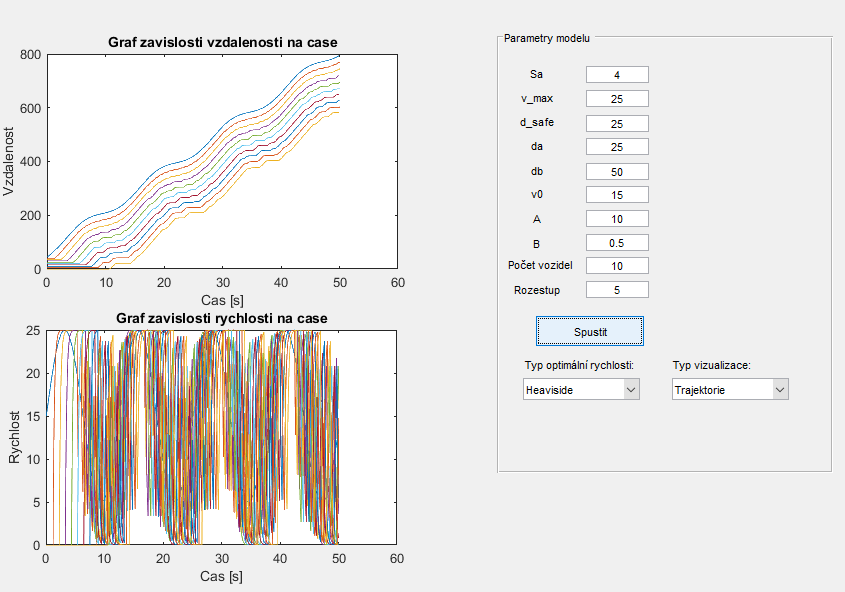
\includegraphics[width=\textwidth]{images/gui.png}
	\caption{Ukázka GUI.}
	\label{Obr: GUI}
\end{figure}


\pagebreak
\section{Výsledky a diskuze}

\subsection{Trajektorie}

Nejprve se podíváme na porovnání trajektorií vozidel. V obrázku \ref{Obr: Trajektorie 1} si můžeme všimnout, že změny rychlosti jsou výrazné, proto v trajektoriích jednotlivých vozidel vidíme spoustu ostrých zubů, které vyznačují skokové zpomalování i zrychlování. To bychom od funkce $\vopt^{(1)}$ přesně očekávali. Navíc si můžeme všimnout, že v určitých chvílích dochází k úplnému zastavení vozidel, kdy se jejich poloha nemění.

Jiná situace nastává na obrázcích \ref{Obr: Trajektorie 2} a \ref{Obr: Trajektorie 3}. U funkce $\vopt^{(2)}$ s lineární složkou vidíme, že každé vozidlo přímo reaguje na vozidlo přes sebou. Vidíme tak plynulý provoz, který naznačuje ideální chování řidičů. Samozřejmě tato situace neodpovídá realitě, kdy jednotliví řidiči nereagují okamžitě (jak můžeme vidět zde), ale jejich reakce je zpomalená o reakční dobu. Funkce  $\vopt^{(2)}$ obsahuje čtvrtou mocninu rozdílu vzdálenosti $\Delta x$. Jejich zrychlování je pomalejší než u předchozí funkce, což má za následek postupné zpomalování vozidel. V obrázku \ref{Obr: Trajektorie 3} si můžeme všimnout, že 2. a 3. vozidlo reagují téměř bez problému, ale už 10. vozidlo musí při počátku zpomalování leadera úplně zastavit. Stejně tak pak zastavují všechna vozidla za ním a v případě vyššího počtu vozidel by se v tomto případě již tvořila kolona.

Nakonec se dostáváme k $\vopt^{(4)}$, trajektorie lze vidět na Obr. \ref{Obr: Trajektorie 4}. Změny rychlostí vozidel jsou v tomto případě velmi rychlé, tedy můžeme znovu vidět \uv{zubaté} chování trajektorií a velmi brzy i úplné zastavení některých vozidel.

\begin{figure}
	\centering
	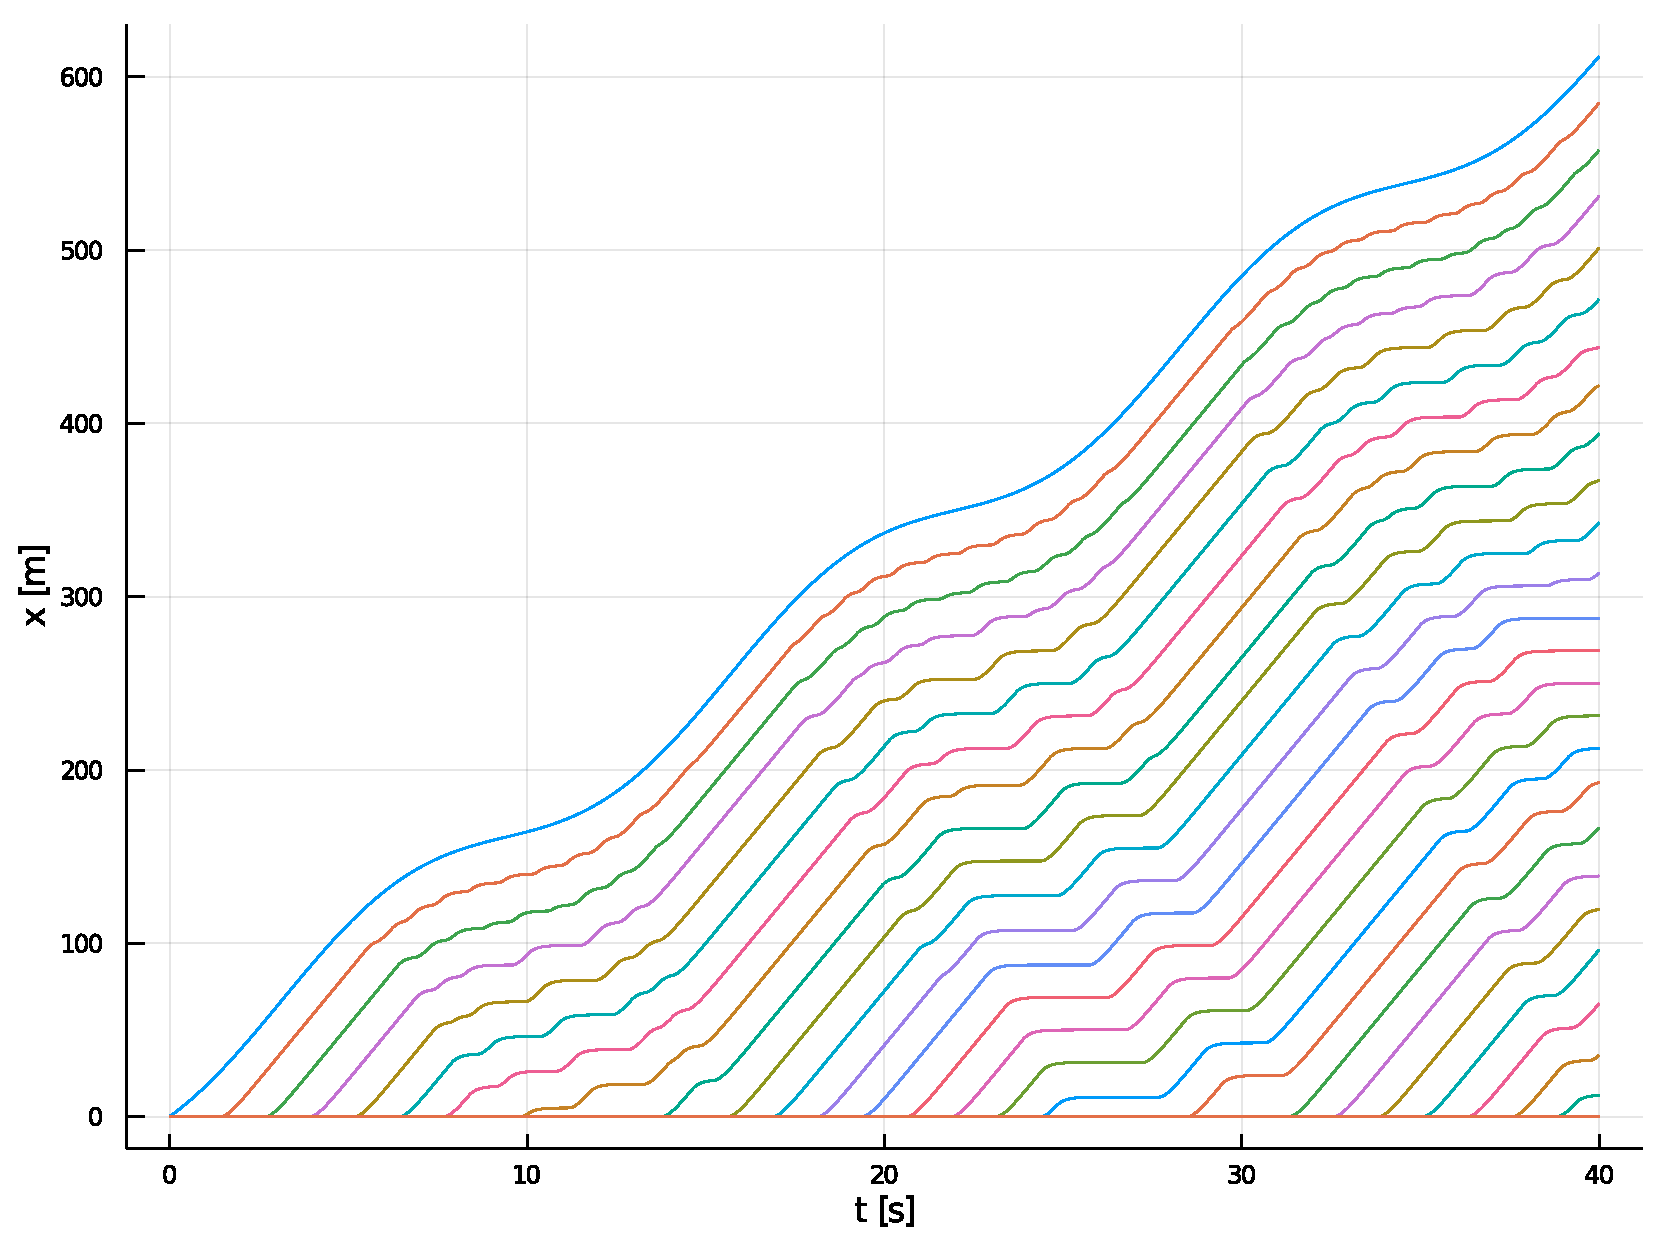
\includegraphics[width=0.9\textwidth]{images/trajektorie_1.pdf}
	\caption{Trajektorie částic pro $\vopt^{(1)}$.}
	\label{Obr: Trajektorie 1}
\end{figure}

\begin{figure}
	\centering
	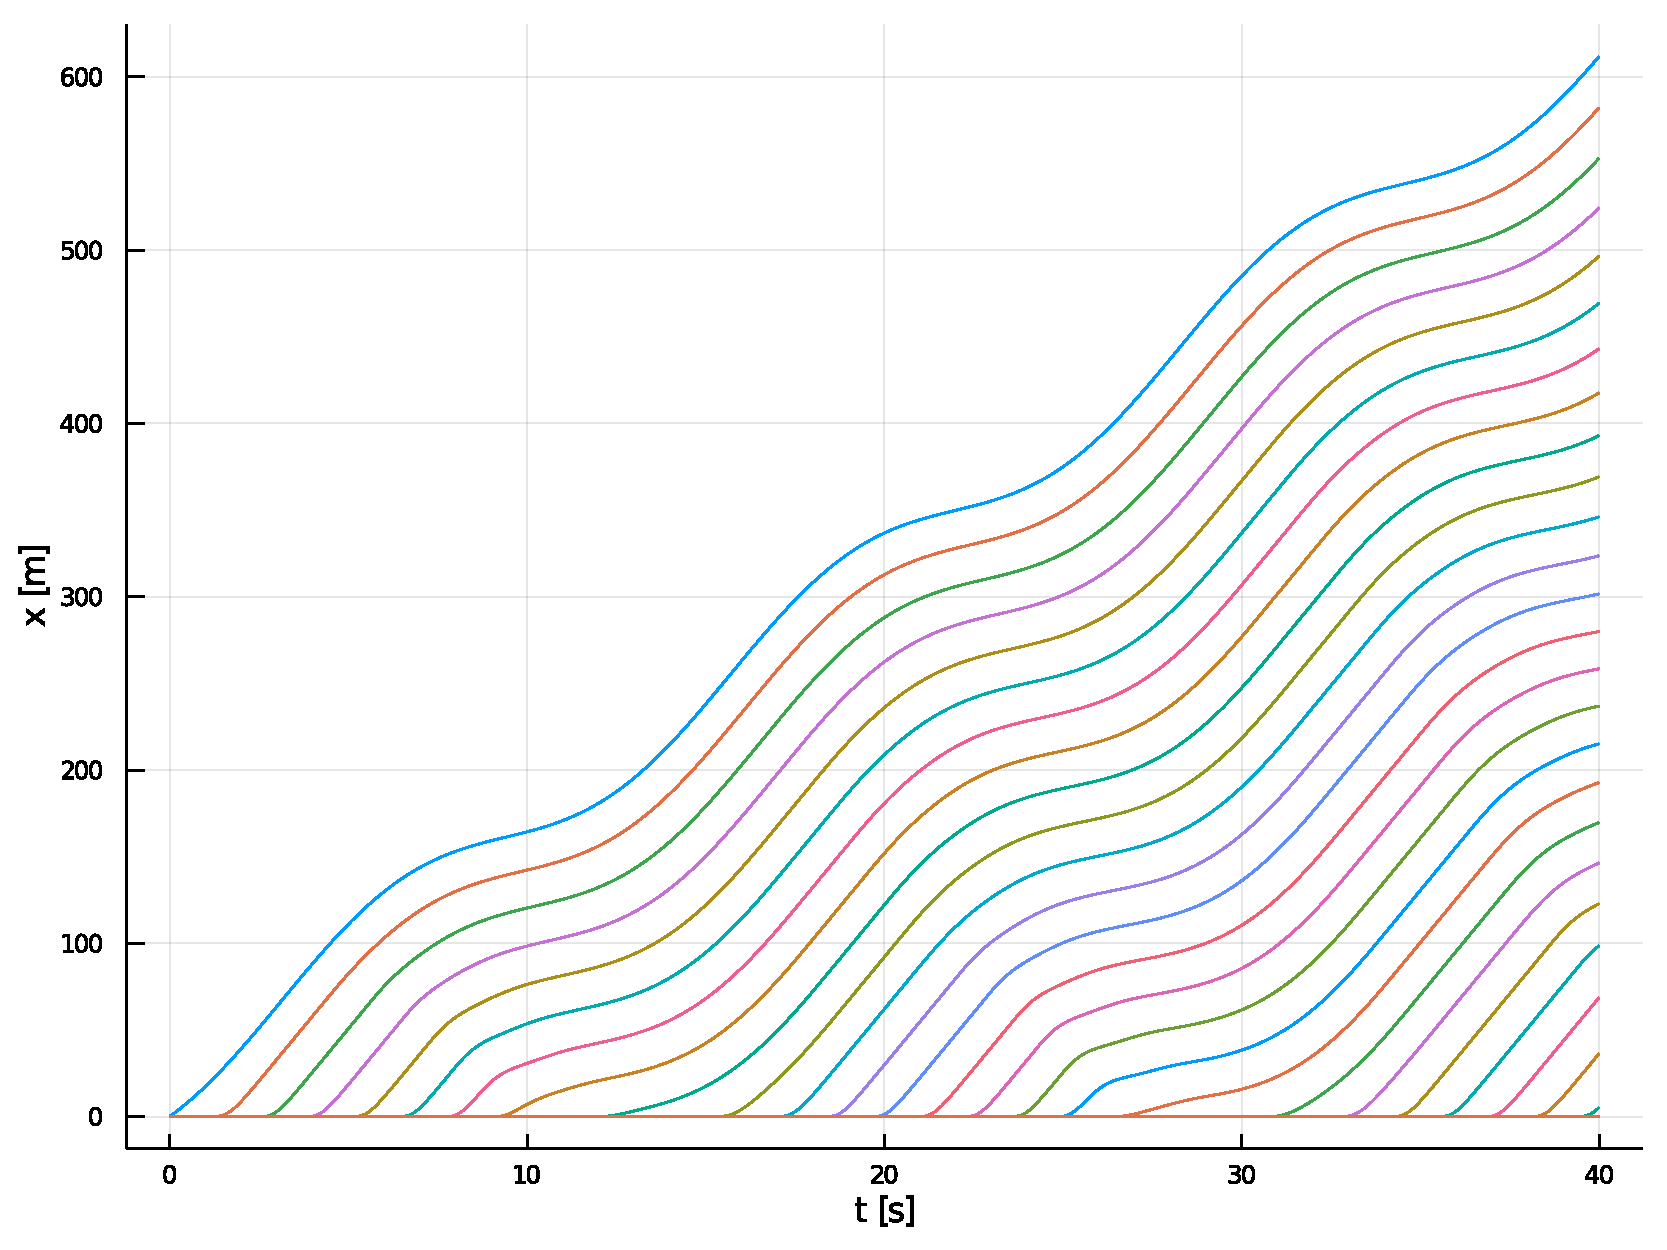
\includegraphics[width=0.9\textwidth]{images/trajektorie_2.pdf}
	\caption{Trajektorie částic pro $\vopt^{(2)}$.}
	\label{Obr: Trajektorie 2}
\end{figure}

\begin{figure}
	\centering
	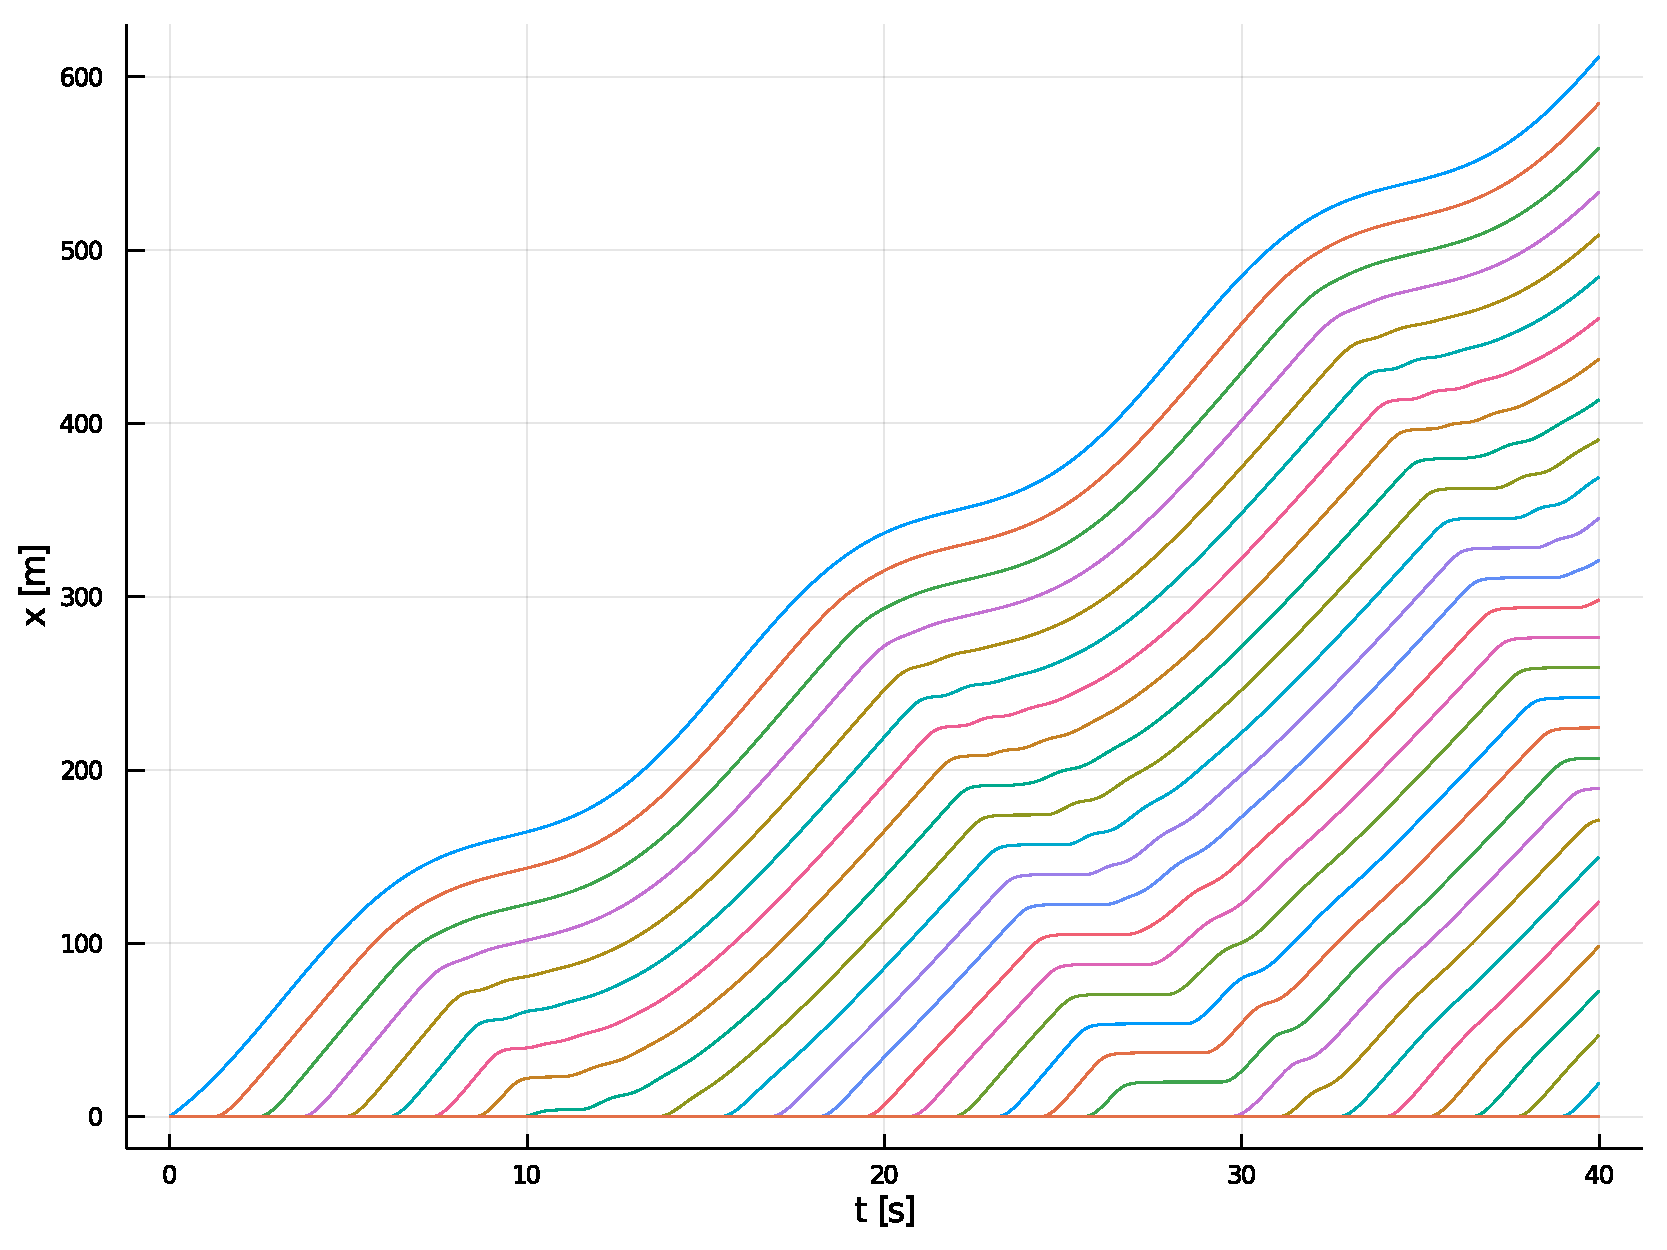
\includegraphics[width=0.9\textwidth]{images/trajektorie_5.pdf}
	\caption{Trajektorie částic pro $\vopt^{(3)}$.}
	\label{Obr: Trajektorie 3}
\end{figure}

\begin{figure}
	\centering
	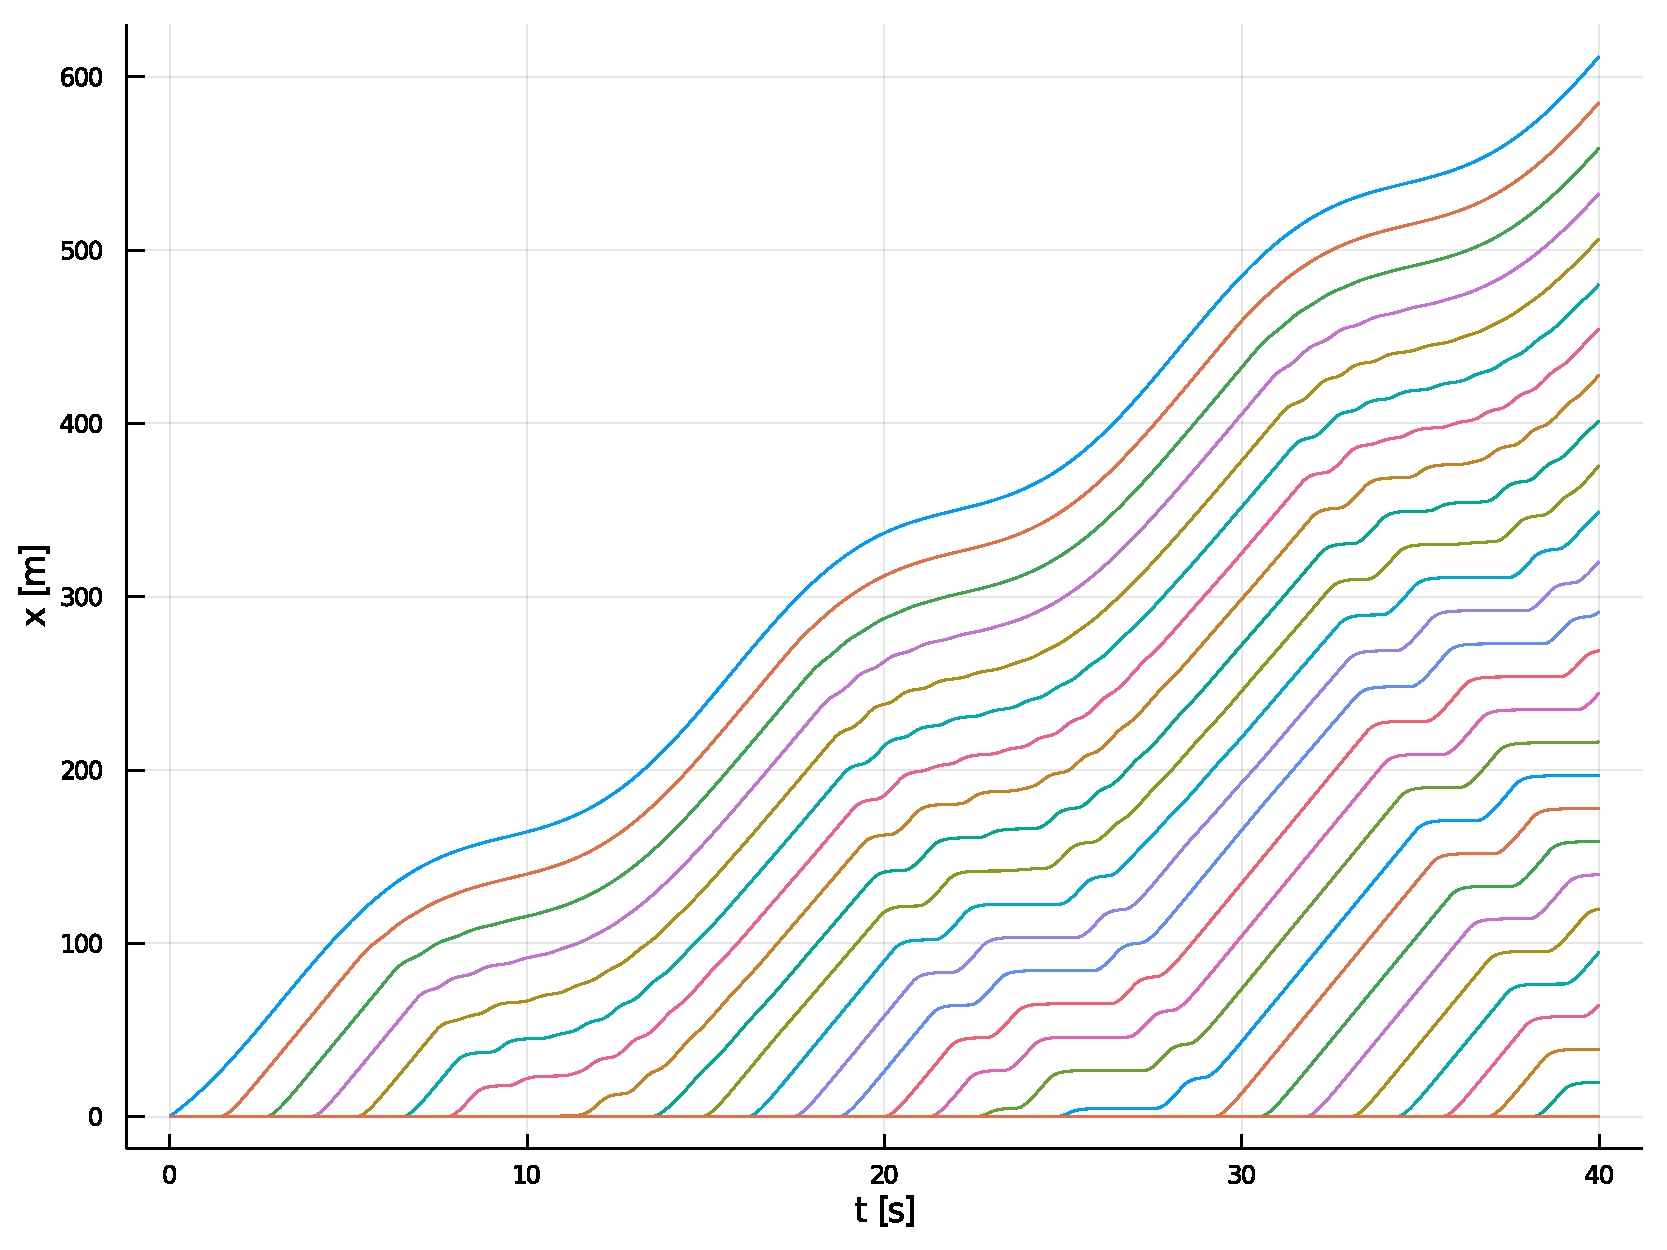
\includegraphics[width=0.9\textwidth]{images/trajektorie_3.pdf}
	\caption{Trajektorie částic pro $\vopt^{(4)}$.}
	\label{Obr: Trajektorie 4}
\end{figure}

\subsection{Fundamentální diagram}

Dále nás zajímají fundamentální diagramy. Ty byly tvořeny pro různý počet částic od 2 do 100. Hodnota pro daný počet částic je tak vyznačena barevným gradientem. U všech diagramů si můžeme všimnou určité konvergence ke kombinaci fundamentálních veličin při zvyšujícím se počtu částic v systému. U všech diagramů platí, že pro velmi nízký počet částic (cca 5-10) se hodnoty pohybují určitým směrem, než začnou sledovat daný trend. Pro více než 10 částic pak tok zůstává víceméně konstantní.

Pro $\vopt^{(1)}$ je fundamentální diagram na  Obr. \ref{Obr: FD vopt1}. Tok nejdříve lineárně roste a následně zůstává převážně konstantní. To stejné platí pro průměrnou rychlost i hustotu. Velmi zajímavá situace nastává pro $\vopt^{(2)}$. Na Obr. \ref{Obr: FD vopt2} vidíme, že závislost veličin sleduje tvar sinusoidy leadera. Naopak u $\vopt^{(3)}$ můžeme na Obr. \ref{Obr: FD vopt3} sledovat jistou skokovou změnu hodnot jednotlivých veličin. %CO TO ZNAMENÁ?

Nakonec si můžeme prohlédnout fundamentální diagramy pro $\vopt^{(4)}$ na Obr. \ref{Obr: FD vopt4}. I zde si můžeme pro vyšší počet částic všimnout skokových změn.

\begin{figure}
	\centering
	\begin{minipage}[c]{0.7\textwidth}
		\centering
		\vspace*{\fill}
		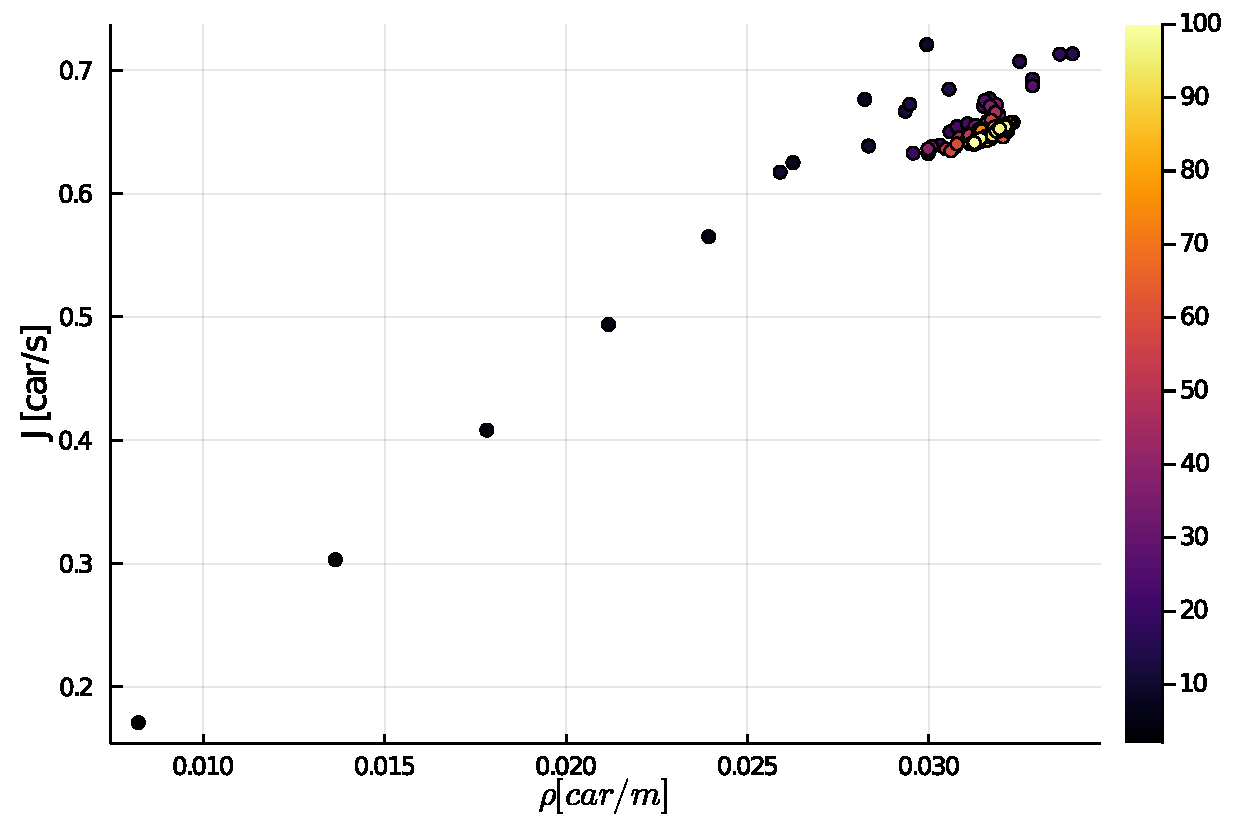
\includegraphics[width=\textwidth]{images/FD_RJ_vopt1.pdf}
		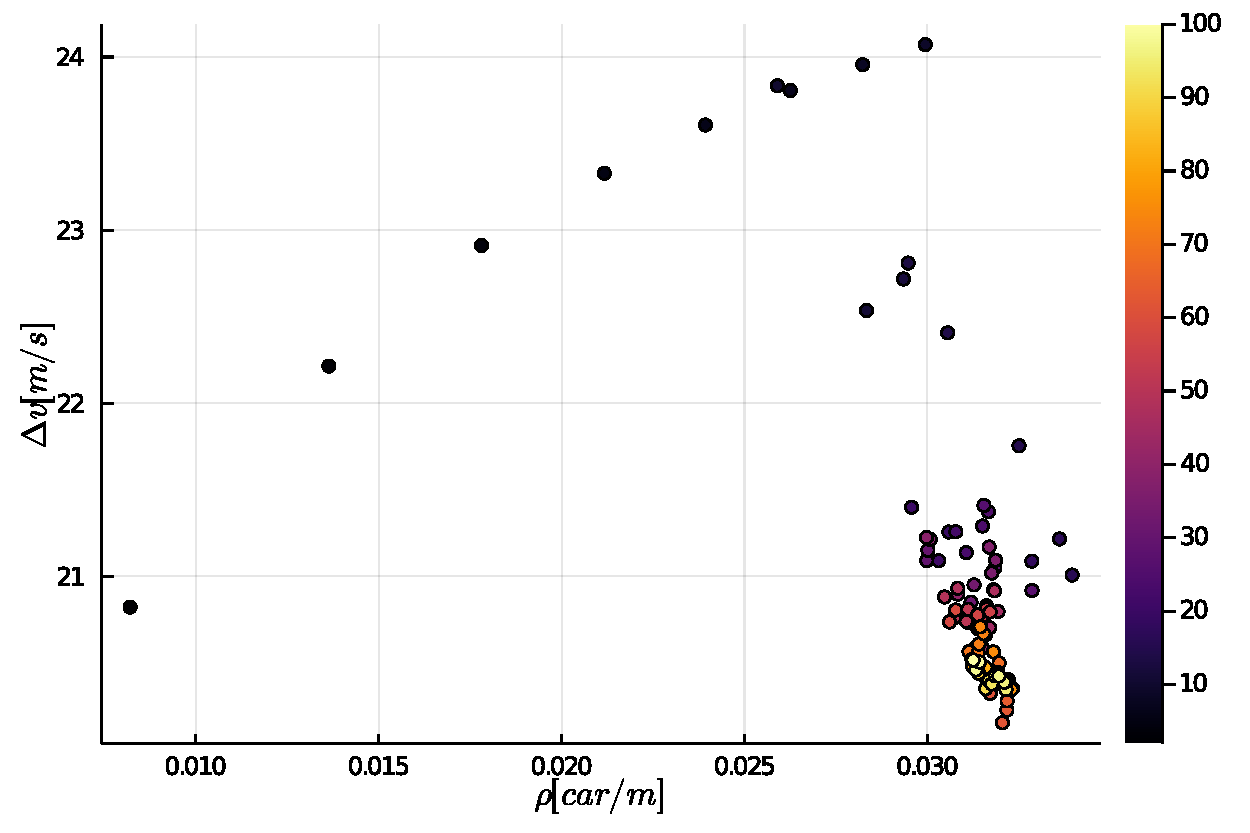
\includegraphics[width=\textwidth]{images/FD_RV_vopt1.pdf}
		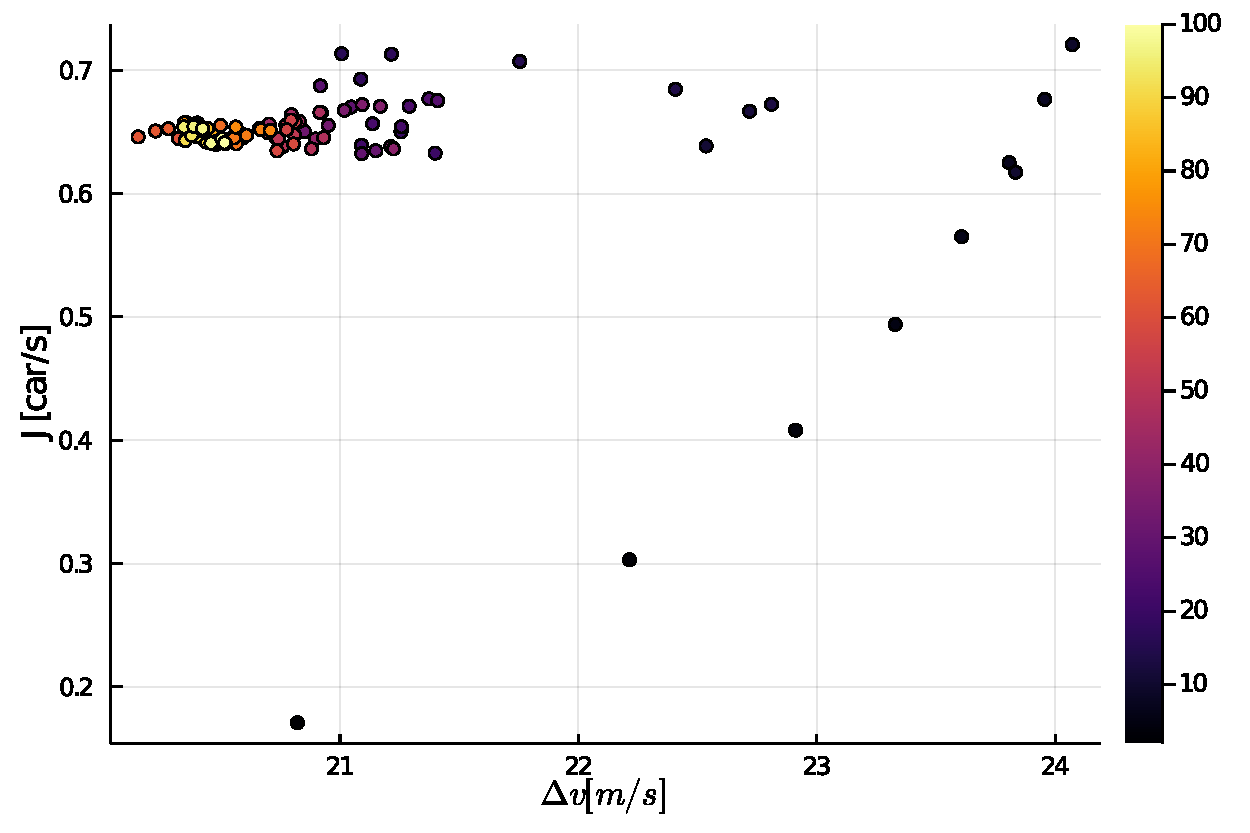
\includegraphics[width=\textwidth]{images/FD_VJ_vopt1.pdf}
	\end{minipage}
	\caption{Fundamentální diagram pro $\vopt^{(1)}$.}
\label{Obr: FD vopt1}
\end{figure}

\begin{figure}
	\centering
	\begin{minipage}[c]{0.7\textwidth}
		\centering
		\vspace*{\fill}
		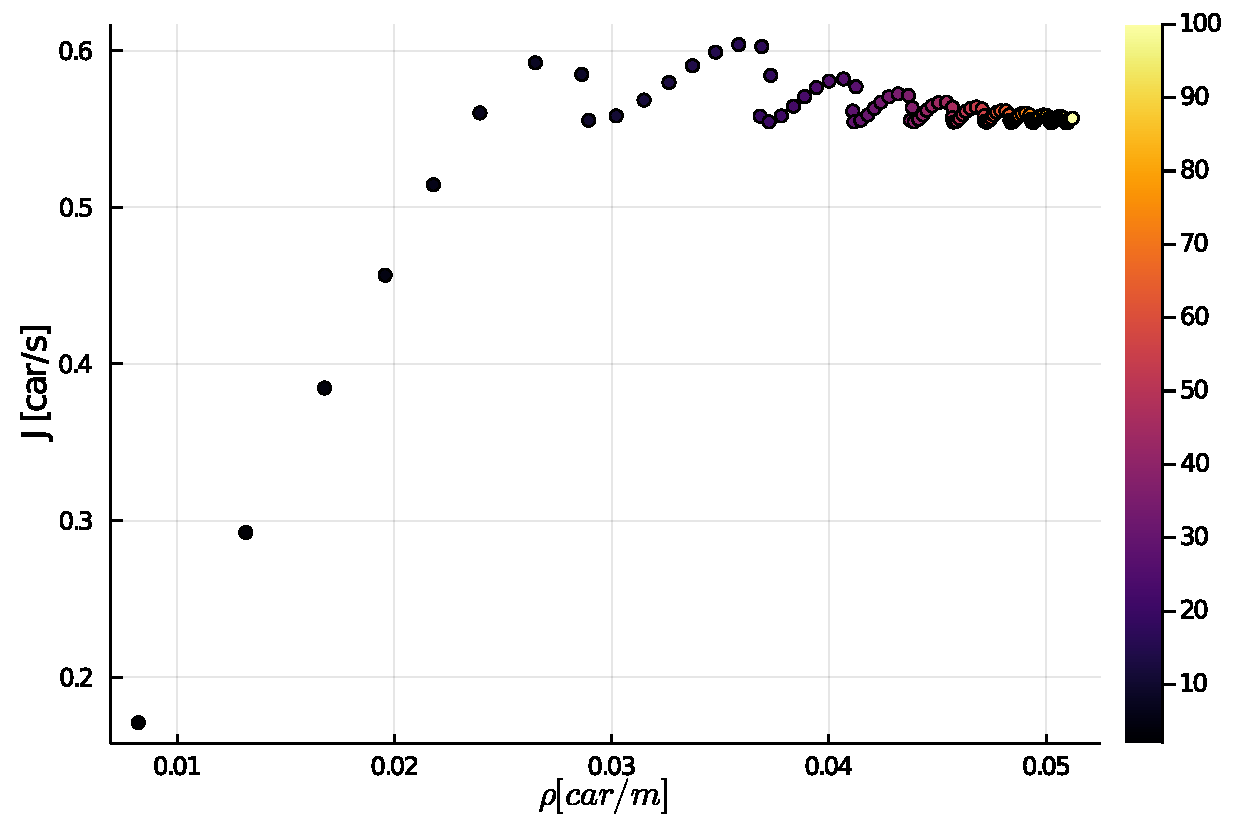
\includegraphics[width=\textwidth]{images/FD_RJ_vopt2.pdf}
		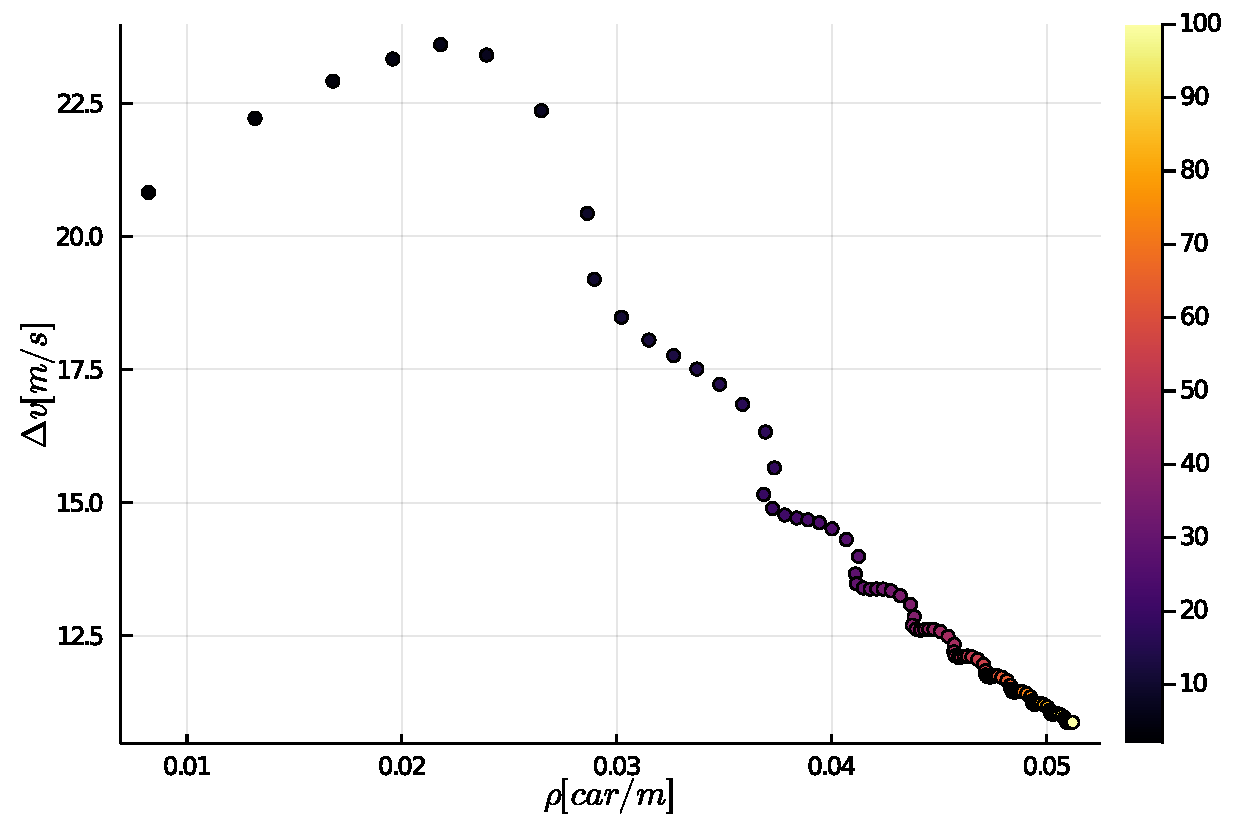
\includegraphics[width=\textwidth]{images/FD_RV_vopt2.pdf}
		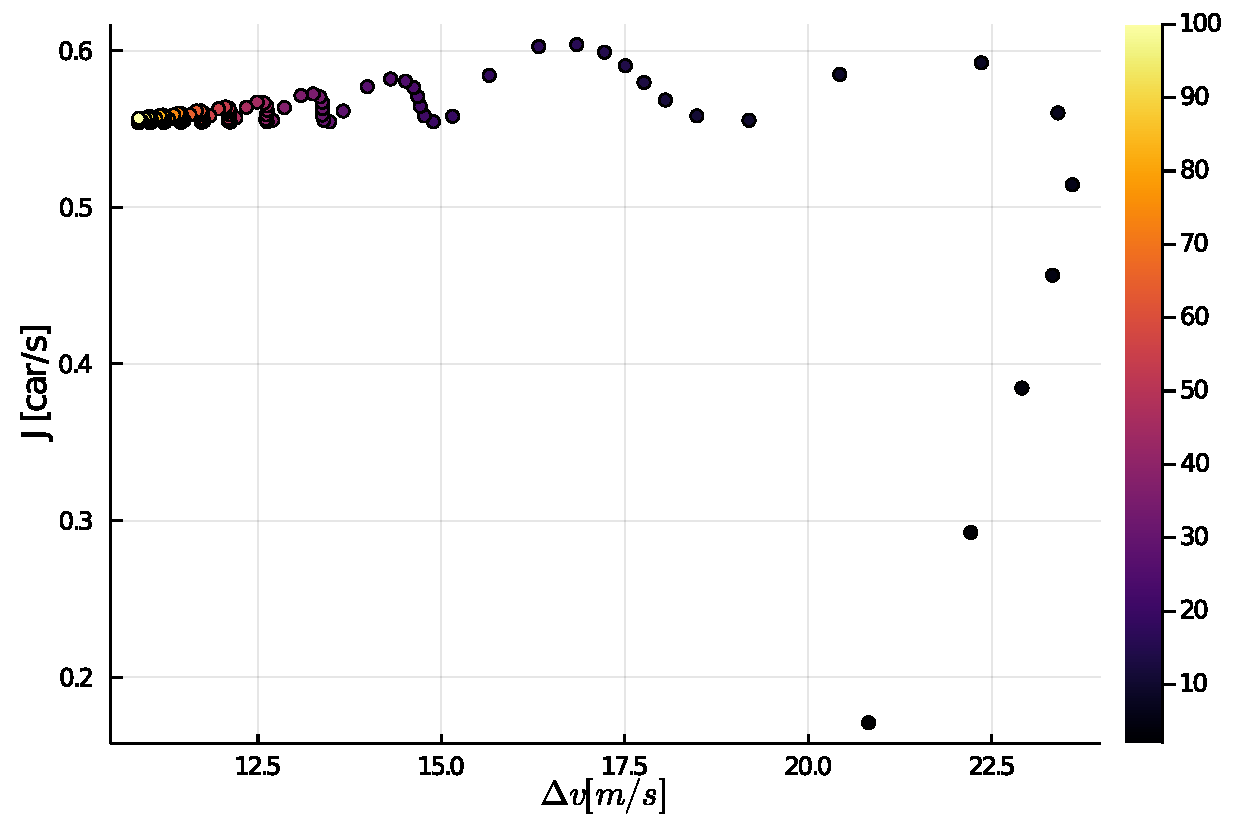
\includegraphics[width=\textwidth]{images/FD_VJ_vopt2.pdf}
	\end{minipage}
	\caption{Fundamentální diagram pro $\vopt^{(2)}$.}
	\label{Obr: FD vopt2}
\end{figure}

\begin{figure}
	\centering
	\begin{minipage}[c]{0.7\textwidth}
		\centering
		\vspace*{\fill}
		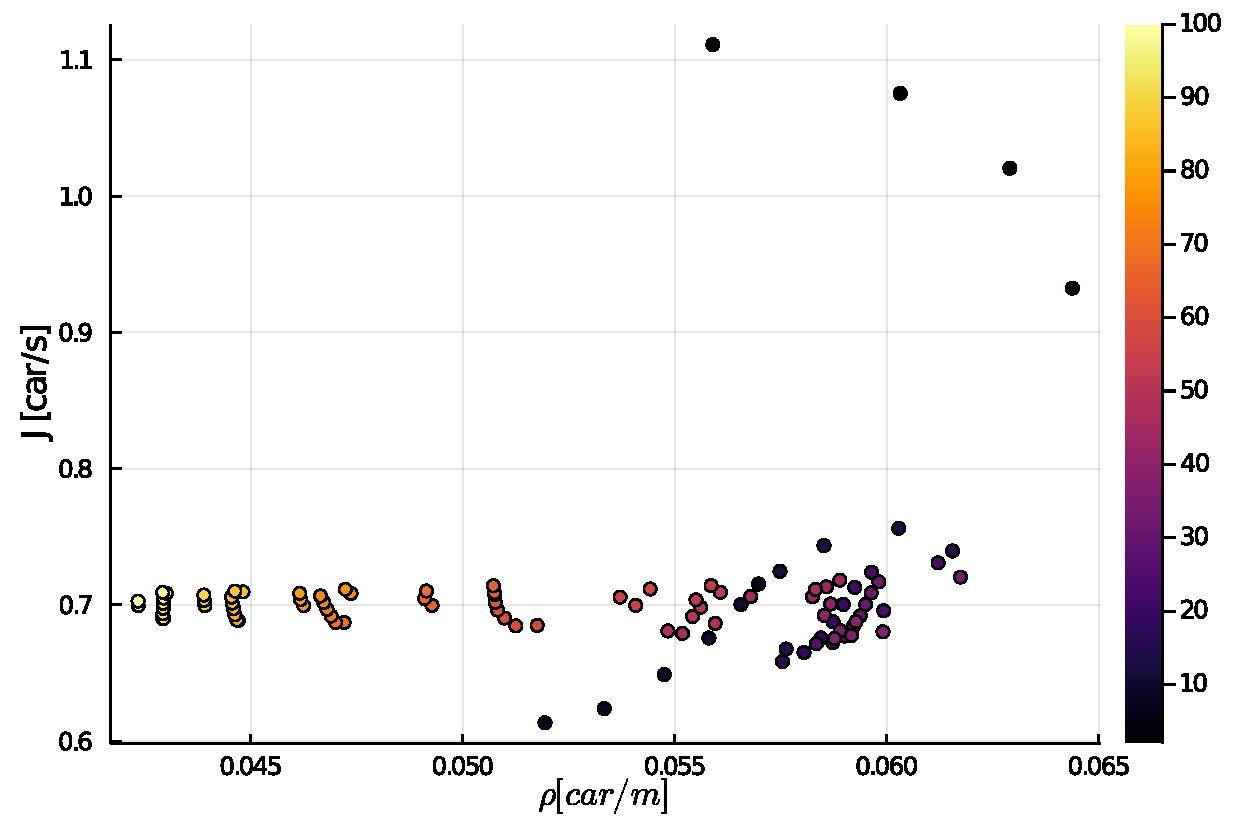
\includegraphics[width=\textwidth]{images/FD_RJ_vopt5.pdf}
		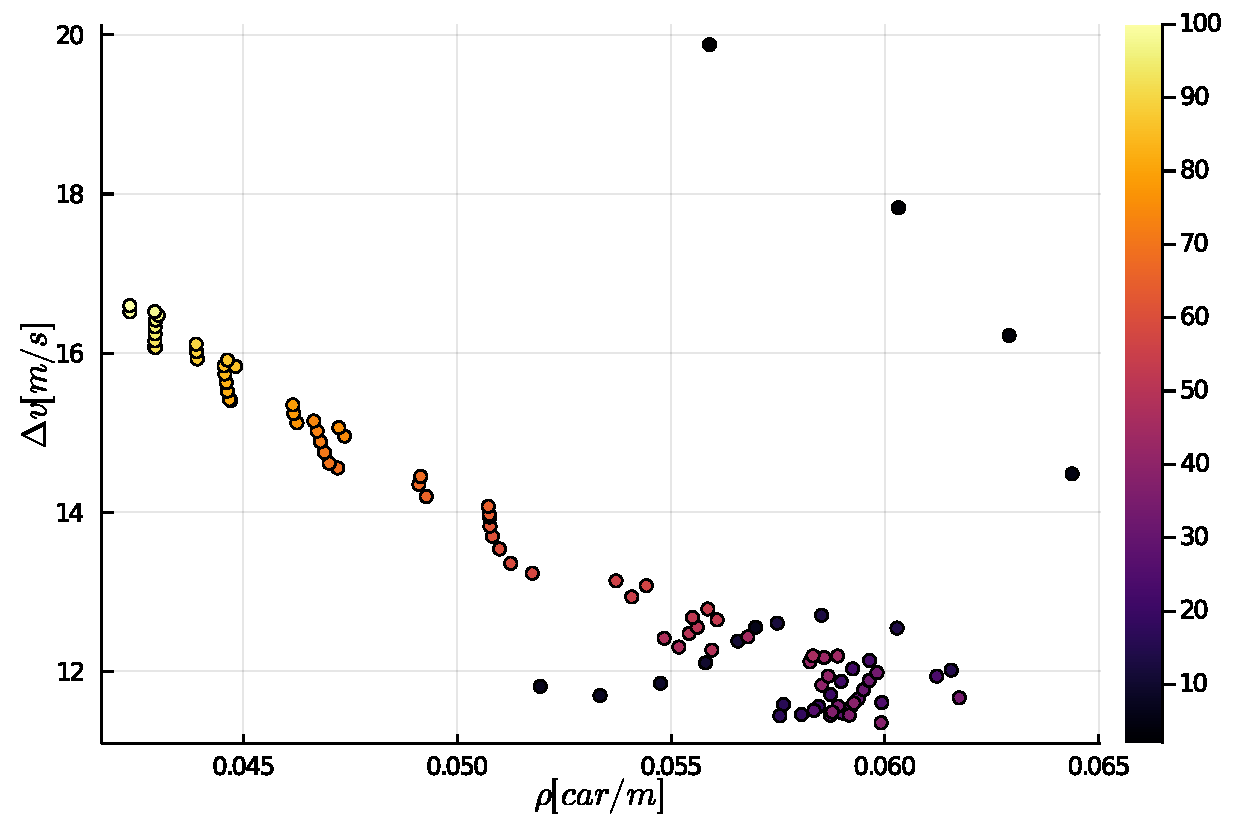
\includegraphics[width=\textwidth]{images/FD_RV_vopt5.pdf}
		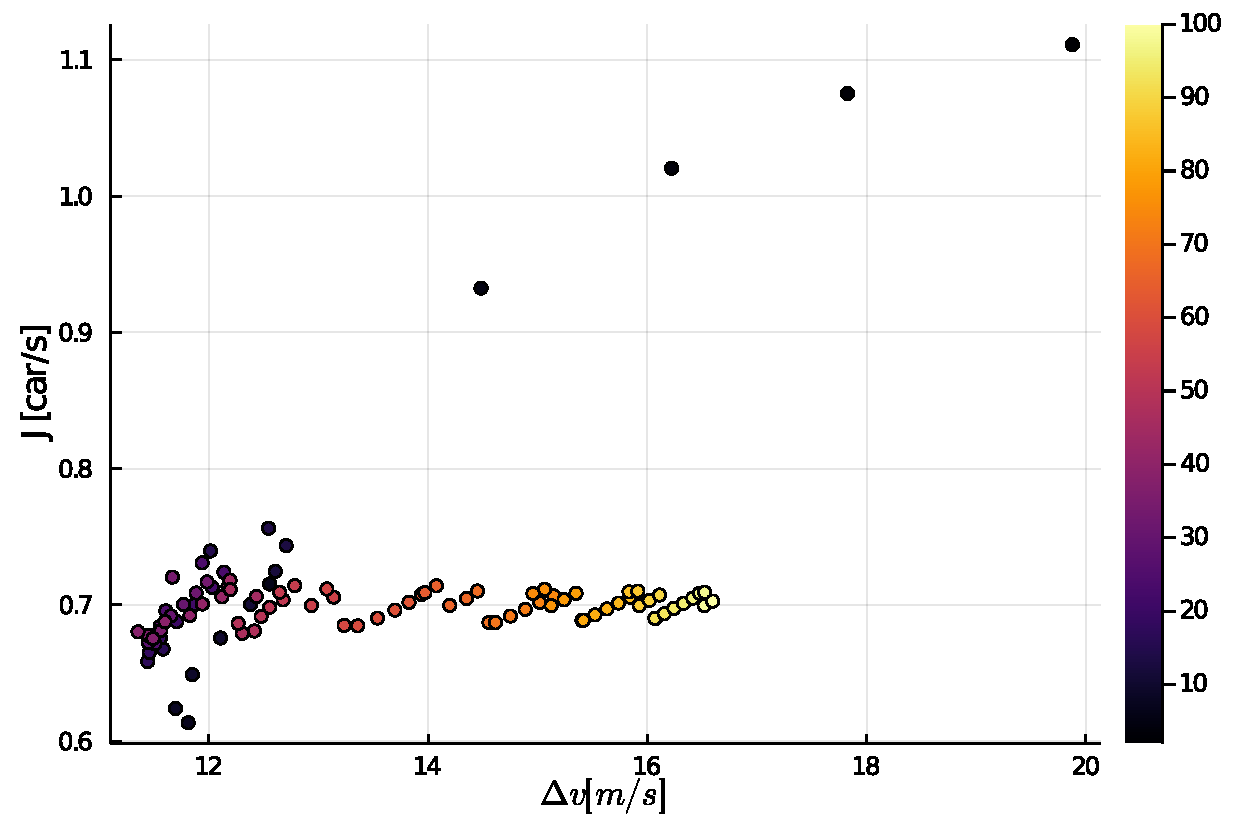
\includegraphics[width=\textwidth]{images/FD_VJ_vopt5.pdf}
	\end{minipage}
	\caption{Fundamentální diagram pro $\vopt^{(3)}$.}
	\label{Obr: FD vopt3}
\end{figure}

\begin{figure}
	\centering
	\begin{minipage}[c]{0.7\textwidth}
		\centering
		\vspace*{\fill}
		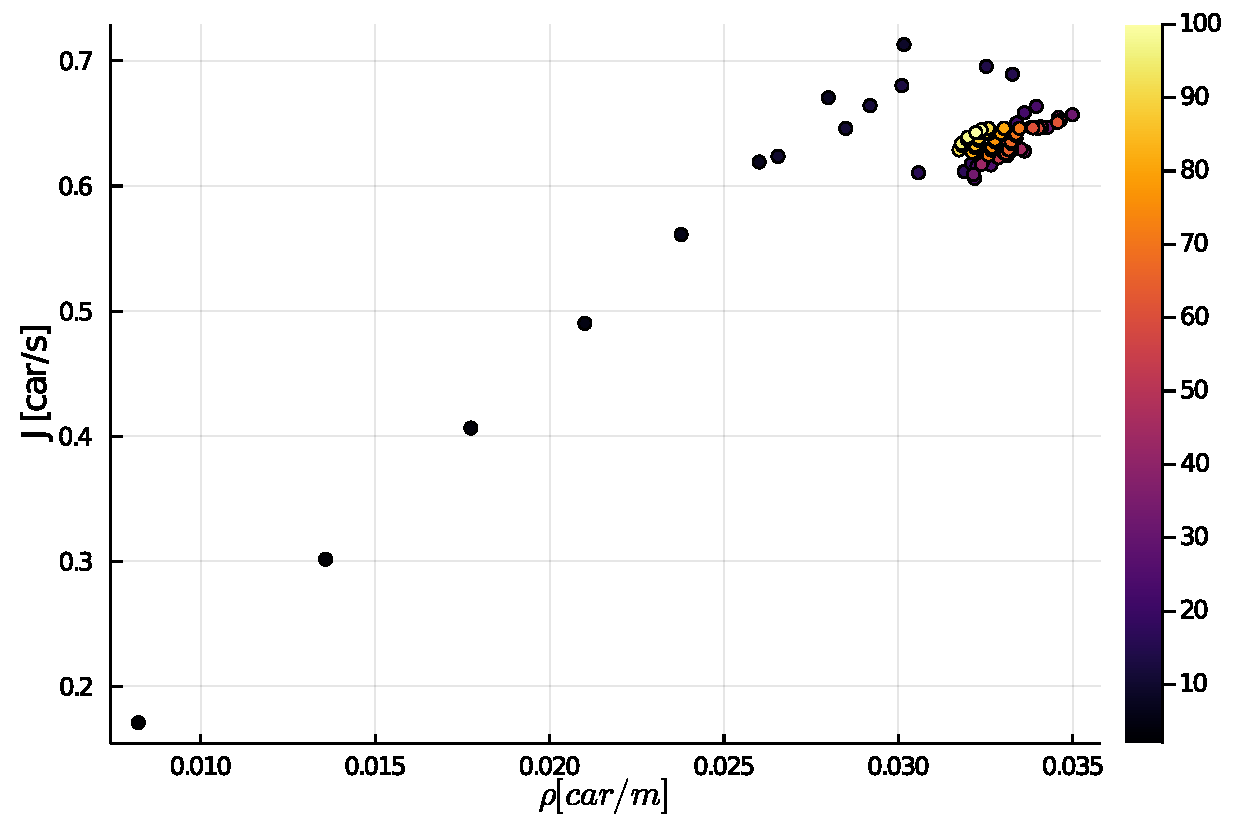
\includegraphics[width=\textwidth]{images/FD_RJ_vopt3.pdf}
		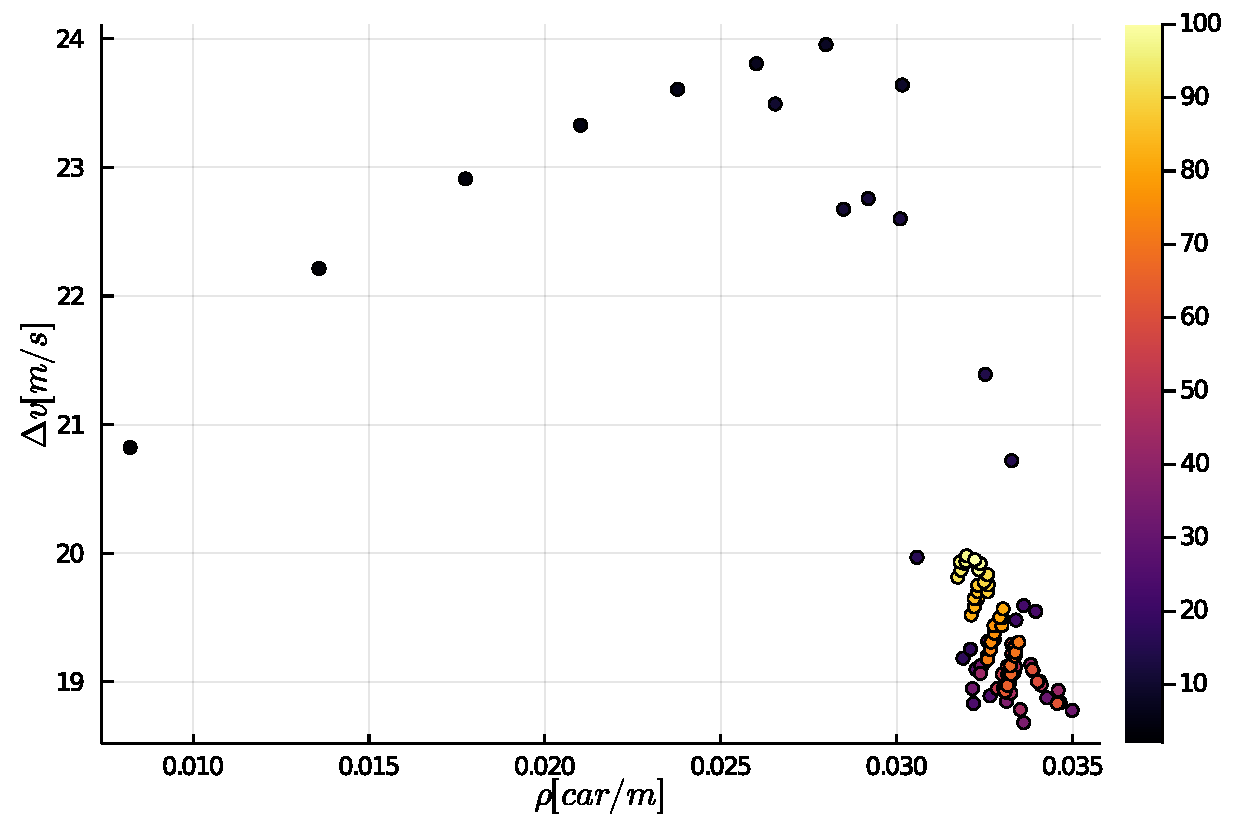
\includegraphics[width=\textwidth]{images/FD_RV_vopt3.pdf}
		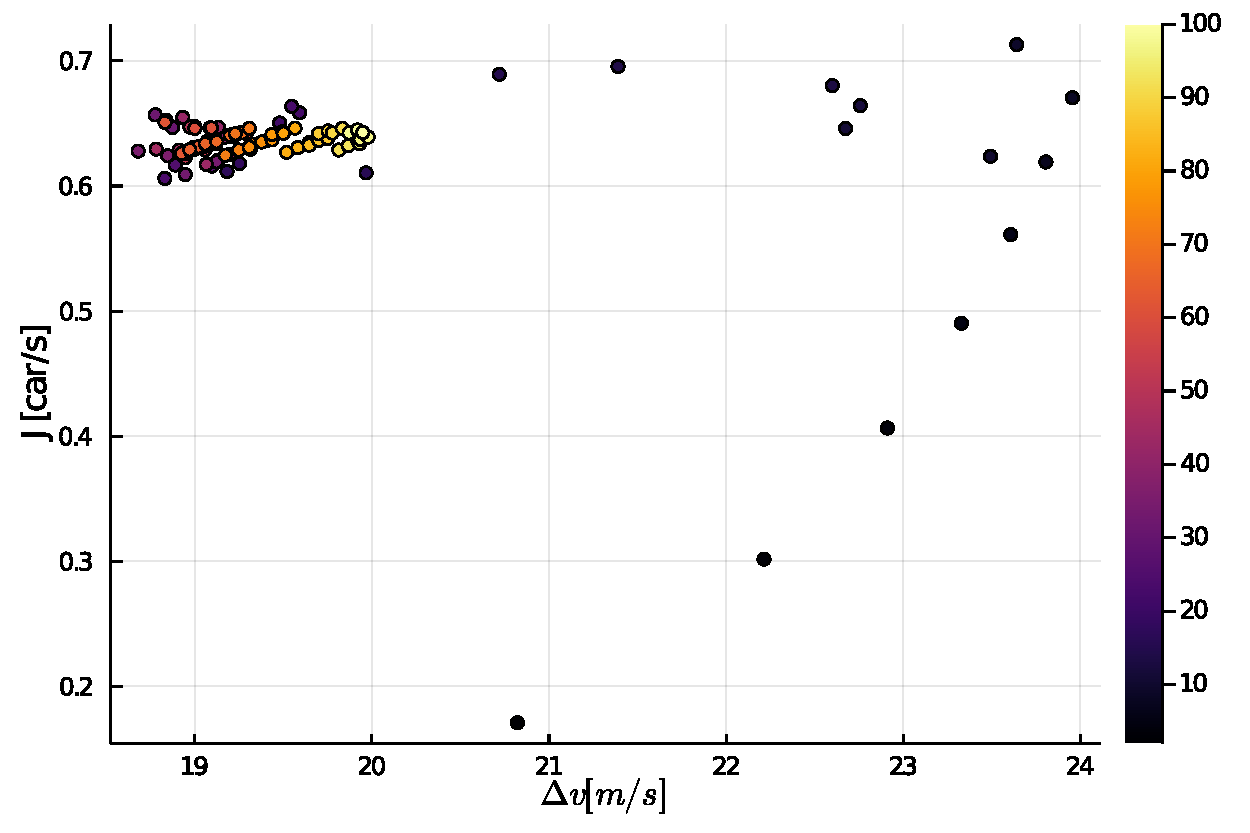
\includegraphics[width=\textwidth]{images/FD_VJ_vopt3.pdf}
	\end{minipage}
	\caption{Fundamentální diagram pro $\vopt^{(4)}$.}
	\label{Obr: FD vopt4}
\end{figure}

%TADY JE POTŘEBA TO ROZMYSLET. ASI TO TOTIŽ NEDÁVÁ SMYSL TÍM, ŽE JE TO POLOHOVÝ TRIGGER TEDY TAM TY AUTA JEDOU RYCHLOSTÍ PODLE LEADERA. ALE MOŽNÁ TO SMYSL DÁVÁ, TEĎ SE NEDOKÁŽU ROZHODNOUT :D

Nakonec porovnáme jednotlivé fundamentální veličiny v tabulce pro počet částic \linebreak $N = 100$. Maximální hodnota pro každou veličinu je vyznačena tučně. Nejvyšší průměrné rychlosti dosahuje model s $\vopt^{(1)}$. To je pravděpodobně způsobeno možností skokově měnit rychlost, tedy případné zrychlení na $\vmax$ je okamžité a je možné tak dosáhnout nejvyšší průměrné rychlosti. Na druhém místě se umístila funkce $\vopt^{(4)}$, která více odpovídá reálnému chování v provozu. Naopak nejnižší je průměrná rychlost pro model s $\vopt^{(2)}$. Vidíme tedy, že částice se sice pohybují synchronně, ale v průměru při průjezdu detektorem dosahují nízkých rychlostí. Nejvyšší tok vidíme pro $\vopt^{(3)}$. 

\begin{table}[h]
	\centering
	\begin{tabular}{rrrr}
		\toprule
			 			& $J [\mathrm{car}/m]$ 	& $\Delta v [m/s]$ 	& $\rho [\mathrm{car}/m]$ \\ \midrule
		$\vopt^{(1)}$	& 0.64 					& \textbf{20.52}	& 0.03 \\ \midrule 
		$\vopt^{(2)}$	& 0.56					& 10.88				& \textbf{0.05} \\ \midrule
		$\vopt^{(3)}$	& \textbf{0.70}			& 16.60				& 0.04 \\ \midrule
		$\vopt^{(4)}$	& 0.64					& 19.95				& 0.03 \\ \bottomrule
	\end{tabular}
\end{table}

\pagebreak
\section{Závěr}

V protokolu se ukázalo, že volba funkcí optimální rychlosti má vliv na chování celého systému. Jako nejideálnější se ukázala funkce $\vopt^{(2)}$, která měla lineární složku. Jednalo se o jedinou funkci, kde nedocházelo k úplnému zastavení některých vozidel. Nicméně tato funkce neodpovídá realitě.

Zároveň se projevila důležitost správného nastavení konstanty $\Sa$ v modelu. V případě nesprávně zvolených hodnot totiž může dojít k nefunkčnosti celé simulace, protože jednotlivé částice nedokážou dostatečně rychle reagovat (brzdit). Například pro hodnotu $\Sa < 1$ pak u některých optimálních funkcí docházelo k nefunkčnosti simulace.

Ve fundamentálních diagramech se projevilo, že pro zvyšující se počet vozidel jednotlivé veličiny konvergují a tok se stane víceméně konstantním. Toto chování však může být dáno i tím, že Optimal velocity model není dostačující pro popis reálného silničního provozu.

Pro 100 částic v systému byly navíc spočteny hodnoty jednotlivých fundamentálních veličin. Ukázalo se, že nejvyšší průměrné rychlosti bylo dosaženo pro $\vopt^{(1)}$, nejspíše proto, že pro tuto optimální rychlost se rychlost vozidel mění skokově a dokáže velmi rychle reagovat na změny. Hned na druhém místě pak byla funkce $\vopt^{(4)}$, která by měla nejvíce odpovídat reálnému provozu.

\end{document}